% Vorbereitung: Vorbereitungsaufgaben bearbeiten
% Versuchsaufbau: Verwendete Apparatur, Beschreibung Funktionsweise/Nutzen mit Skizze/Foto
\section{Durchführung}
\label{sec:durchführung}

Der verwendete Aufbau lässt sich anhand Abbildung \ref{fig:aufbau} nachvollziehen. Nachdem am Plattenkondensator eine feste Spannung $U$
eingestellt ist, mithilfe derer sich über $U = dE$ die Feldstärke ermitteln lässt, wird im zunächst feldfreien Zwischenraum der Höhe $d$
Öl zerstäubt. Aus der Menge der so entstehenden Tröpfchen lassen sich durch kurzes Einschalten des elektrischen Feldes solche identifizieren,
die als Resultat der Reibung bei der Injektion eine Ladung besitzen. Anchließend werden je die Zeiten $t_0$ ohne Feld sowie $t_\text{auf}$ und
$t_\text{ab}$ bei entsprechender Polung gemessen, welche das Tröpfchen benötigt, um eine Distanz $s$ zurückzulegen. Mittels $s = vt$ ergeben
sich damit die Geschwindigkeiten zur weiteren Rechnung. Für jeden gewählten Öltropfen werden außerdem Spannung und Thermistor-Widerstand
an den jeweiligen Buchsen abgegriffen und geprüft. Aus dem Widerstand $R$ wird mithilfe einer Tabelle die vorherrschende Temperatur $T$ bestimmt,
welche sich durch die Halogenlampe zur Erleuchtung der Kondensatorkammer graduell erhöht. Bei Normaldruck $p$ lassen sich auf diese Weise
Viskosität $\eta_L$ und Dichte $\rho_L$ von Luft ermitteln. Dieses Vorgehen wird mehrfach für verschiedene Tröpfchen wiederholt, zur besseren
Vergleichbarkeit ist die Hälfte der Messreihe für eine von der ersten abweichende Feldspannung aufgenommen. Das zur Ionisation der Umgebungsluft
verbaute schwach radiaktive Thorium-Präparat bleibt abgeschirmt.

Aus den so gewonnenen Werten werden unter Anwendung der zuvor beschriebenen mathematischen Zusammenhänge die korrigierten Ladungen $q$ der
Öltröpfchen bestimmt. Der größte gemeinsame Divisor gibt dann folglich die Elementarladung $e_0$ an.

\begin{figure}[H]
	\centering
	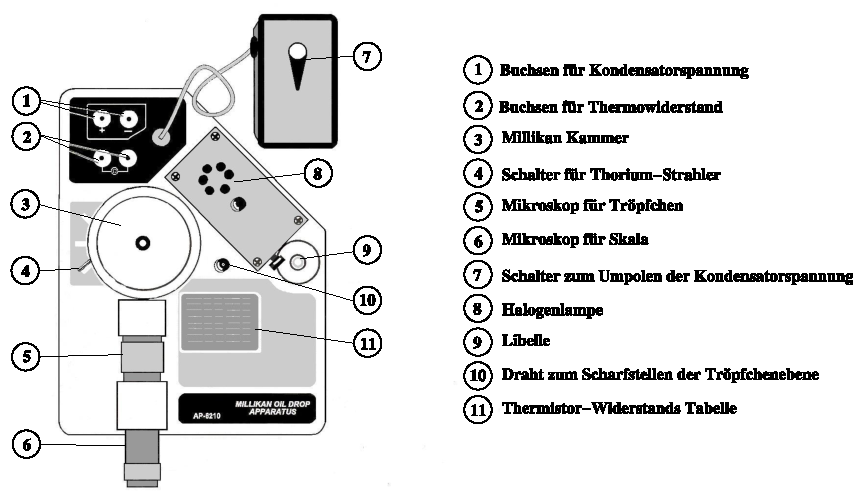
\includegraphics[width=0.95\linewidth]{content/grafik/aufbau.pdf}
	\caption{Schematischer Aufbau der Messapparatur zum Millikan-Versuch.}
	\label{fig:aufbau}
\end{figure}
